\section{Máquinas de Turing}

  % Lemma 79: Nada.
  \begin{lemma}
    \PN Este lemma no se evalua.
  \end{lemma}

	% Lemma 80: Con prueba.
  \begin{lemma}
  	\PN El predicado $\lambda dd^{\prime} \left[d \vdash d^{\prime}\right]$ es $(\Gamma \cup Q)$-PR.
  \end{lemma}
	\begin{proof}
	  \PN Note que $D_{\lambda dd^{\prime}\left[d\ \vdash d^{\prime }\right] }=Des\times Des$. También nótese que los
    predicados
    \begin{eqnarray*}
      \lambda q\sigma p\gamma \left[ (q,\sigma ,L)\in \delta (p,\gamma )\right] \\
      \lambda q\sigma p\gamma \left[ (q,\sigma ,R)\in \delta (p,\gamma )\right] \\
      \lambda q\sigma p\gamma \left[ (q,\sigma ,K)\in \delta (p,\gamma )\right]
    \end{eqnarray*}

    \PN son $(\Gamma \cup Q)$-PR, ya que los tres tienen dominio igual a $Q \times \Gamma \times Q \times \Gamma$ el
    cual es finito por \textbf{Corollary 36}.

    \vspace{3mm}
    \PN Sean:
    \begin{eqnarray*}
      && P_{R}: Des \times Des \times \Gamma \times \Gamma^{\ast} \times \Gamma^{\ast} \times Q \times Q \rightarrow
        \omega \\
      && P_{R}(d,d^{\prime},\sigma,\alpha,\beta,p,q) = 1 \Leftrightarrow \left(d = \alpha p \beta\right) \wedge
        \left((q,\sigma,R) \in \delta \left(p,\left[\beta B\right]_{1}\right)\right) \wedge \left(d^{\prime} =
        \left\lfloor \alpha \sigma q^{\curvearrowright}\beta \right\rfloor\right) \\
      \\
      && P_{L}: Des \times Des \times \Gamma \times \Gamma^{\ast} \times \Gamma^{\ast} \times Q \times Q \rightarrow
        \omega \\
      && P_{L}(d,d^{\prime},\sigma,\alpha,\beta,p,q) = 1 \Leftrightarrow \left(d = \alpha p \beta \right) \wedge
        \left((q,\sigma,L) \in \delta \left(p,\left[\beta B\right]_{1}\right)\right) \wedge \left(\alpha \neq
        \varepsilon\right) \wedge \left(d^{\prime} = \left\lfloor \alpha^{\curvearrowleft} q \left[\alpha\right]_{\lvert
        \alpha \rvert} \sigma^{\curvearrowright} \beta \right\rfloor\right) \\
      \\
      && P_{K}: Des \times Des \times \Gamma \times \Gamma^{\ast} \times \Gamma^{\ast} \times Q \times Q \rightarrow
        \omega \\
      && P_{K}(d,d^{\prime},\sigma,\alpha,\beta,p,q) = 1 \Leftrightarrow \left(d = \alpha p \beta\right) \wedge
        \left((q,\sigma,K) \in \delta \left(p,\left[\beta B\right]_{1}\right)\right) \wedge \left(d^{\prime} =
        \left\lfloor \alpha q \sigma^{\curvearrowright} \beta \right\rfloor\right)
      \end{eqnarray*}
    \PN Veamos, por ejemplo, que $P_L$ es $(\Gamma \cup Q)$-PR. Notar que:
    \[
      P_L = P_1 \land P_2 \land P_3 \land P_4
    \]

    \PN donde $P_1, P_2,  P_3, P_4$ son los siguientes predicados:
    \begin{eqnarray*}
      P_1 &=& \lambda dd^{\prime}\sigma\alpha\beta pq \left[d = \alpha p \beta\right] \\
          &=& \lambda \alpha\beta\left[\alpha = \beta\right]
                \circ (
                  p_{1}^{0,7},
                  \lambda \alpha_1\alpha_2\alpha_3\left[\alpha_1\alpha_2\alpha_3\right]
                    \circ (
                      p_{4}^{0,7},
                      p_{6}^{0,7},
                      p_{5}^{0,7})) \\
      \\
      P_2 &=& \lambda dd^{\prime}\sigma\alpha\beta pq \left[(q,\sigma,L) \in \delta \left(p,\left[\beta B\right]_{1}
        \right)\right] \\
          &=& \lambda q\sigma p\gamma \left[(q,\sigma,L) \in \delta (p,\gamma)\right]
                \circ (
                  p_{7}^{0,7},
                  p_{3}^{0,7},
                  p_{6}^{0,7},
                  \lambda i\alpha \left[\left[\alpha\right]_i\right]
                  \circ (
                    C_{1}^{0,7},
                    \lambda \alpha \beta \left[ \alpha\beta \right] \circ (p_{5}^{0,7}, C_{B}^{0,7}))) \\
      \\
      P_3 &=& \lambda d d^{\prime}\sigma\alpha\beta p q \left[ \alpha \neq \varepsilon \right] \\
          &=& \lambda \alpha\beta \left[\alpha \neq \beta\right]
              \circ (
                p_{4}^{0,7},
                C_{\varepsilon}^{0,7}) \\
      \\
      P_4 &=& \lambda dd^{\prime}\sigma\alpha\beta pq \left[d^{\prime} = \left\lfloor \alpha^{\curvearrowleft}q
        \left[\alpha\right]_{\lvert \alpha \rvert } \sigma^{\curvearrowright} \beta \right\rfloor\right] \\
          &=& \lambda \alpha\beta\left[ \alpha=\beta \right]
                \circ (
                  p_{2}^{0,7},
                  \lambda \alpha \left[ \lfloor \alpha \rfloor \right] \circ f) \\
    \end{eqnarray*}
    \PN donde:
    \begin{align*}
      f =  \lambda\alpha_1\alpha_2\alpha_3\alpha_4\alpha_5 \left[ \alpha_1\alpha_2\alpha_3\alpha_4\alpha_5 \right]
            \circ (
              \lambda \alpha \left[ \alpha ^{\curvearrowleft } \right] \circ p_{4}^{0,7},
              p_{7}^{0,7},
              \lambda i\alpha \left[ \left[\alpha\right]_i \right]
                \circ (
                  \lambda \alpha \left[\lvert\alpha\rvert \right] \circ p_{4}^{0,7},
                  p_{4}^{0,7}
              ),
              p_{3}^{0,7},
              \lambda \alpha \left[ ^{\curvearrowright}\alpha \right] \circ p_{5}^{0,7}
            )
    \end{align*}

    \PN Luego, notar que $P_1, P_2 , P_3, P_4 $ son $(\Gamma \cup Q)$-PR, por lo tanto $P_L$ es $(\Gamma \cup Q)$-PR. De
    manera similar, podemos ver que $P_K$ y $P_R$ son $(\Gamma \cup Q)$-PR.

    \PN Tomemos el siguiente predicado:
    \[
      P = (P_{R}\vee P_{L}\vee P_{K})
    \]

    \PN Tenemos que $P$ es $(\Gamma \cup Q)$-PR. Nótese que $\lambda dd^{\prime} \left[d\vdash d^{\prime}\right]$ es
    igual al predicado:
    \begin{eqnarray*}
      \lambda dd^{\prime}\left[(\exists \sigma \in \Gamma)(\exists \alpha,\beta \in \Gamma^{\ast})(\exists p,q \in Q)
      \; P(d,d^{\prime},\sigma,\alpha,\beta,p,q)\right]
    \end{eqnarray*}

    \PN Luego, aplicando cinco veces el \textbf{Lemma 39} obtenemos que $\lambda dd^{\prime} \left[d\vdash d^{\prime}
    \right]$ es $(\Gamma \cup Q)$-PR. Veamos esto. Notar primero que como $\beta, \alpha, \sigma, p, q$ son subpalabras
    de $d$ y $d^{\prime}$ respectivamente, tenemos que $\lvert\beta\rvert, \lvert\alpha\rvert, \lvert\sigma\rvert,
    \lvert p \rvert, \lvert q \rvert \leq \lvert d \rvert + \lvert d^{\prime} \rvert$.
    \begin{align*}
      L_1 &= \lambda xdd^{\prime}\sigma\alpha\beta p \left[(\exists q \in Q)_{\lvert q \rvert \leq x} \; P(d,d^{\prime},
             \sigma,\alpha,\beta,p,q)\right] \\
      Q_1 &= \lambda dd^{\prime}\sigma\alpha\beta p \left[(\exists q \in Q)_{\lvert q \rvert \leq \lvert d \rvert +
             \lvert d^{\prime} \rvert} \; P(d,d^{\prime},\sigma,\alpha,\beta,p,q)\right] \\
          &= L_1 \circ (\lambda xy \left[x + y\right] \circ(\lambda \alpha \left[\lvert\alpha\rvert\right] \circ
             p_{1}^{0,6}, \lambda \alpha \left[\lvert\alpha\rvert\right] \circ p_{2}^{0,6}), p_{1}^{0,6}, p_{2}^{0,6},
             p_{3}^{0,6}, p_{4}^{0,6}, p_{5}^{0,6}, p_{6}^{0,6})
    \end{align*}

    \PN Por \textbf{Lemma 39} tenemos que $L_{1}$ es $(\Gamma \cup Q)$-PR y por ende $Q_{1}$ es $(\Gamma \cup Q)$-PR. De
    la misma manera podemos que el predicado $Q_{2}$ es $(\Gamma \cup Q)$-PR.
    \begin{align*}
      L_2 &= \lambda xdd^{\prime}\sigma\alpha\beta \left[(\exists p \in Q)_{\lvert p \rvert \leq x} \;
             Q_{1}(d,d^{\prime},\sigma,\alpha,\beta,p)\right] \\
      Q_2 &= \lambda dd^{\prime}\sigma\alpha\beta \left[(\exists p \in Q)_{\lvert p \rvert \leq \lvert d \rvert +
             \lvert d^{\prime} \rvert} \; Q_{1}(d,d^{\prime},\sigma,\alpha,\beta,p)\right] \\
          &= L_2 \circ (\lambda xy \left[x + y\right] \circ(\lambda \alpha \left[\lvert\alpha\rvert\right] \circ
             p_{1}^{0,5}, \lambda \alpha \left[\lvert\alpha\rvert\right] \circ p_{2}^{0,5}), p_{1}^{0,5}, p_{2}^{0,5},
             p_{3}^{0,5}, p_{4}^{0,5}, p_{5}^{0,5})
    \end{align*}
    \PN finalmente, tenemos que $Q_{3}, Q_{4}, Q_{5}$ son $(\Gamma \cup Q)$-PR.
    \begin{align*}
      L_3 &= \lambda xdd^{\prime}\sigma\alpha \left[(\exists \beta \in \Gamma^{\ast})_{\lvert\beta\rvert \leq x} \;
             Q_{2}(d,d^{\prime},\sigma,\alpha,\beta)\right] \\
      Q_3 &= \lambda dd^{\prime}\sigma\alpha \left[(\exists \beta \in \Gamma^{\ast})_{\lvert\beta\rvert \leq \lvert d
             \rvert + \lvert d^{\prime} \rvert} \; Q_{2}(d,d^{\prime},\sigma,\alpha,\beta)\right] \\
          &= L_3 \circ (\lambda xy \left[x + y\right] \circ(\lambda \alpha \left[\lvert\alpha\rvert\right] \circ
             p_{1}^{0,4}, \lambda \alpha \left[\lvert\alpha\rvert\right] \circ p_{2}^{0,4}), p_{1}^{0,4}, p_{2}^{0,4},
             p_{3}^{0,4}, p_{4}^{0,4}) \\[10pt]
      L_4 &= \lambda xdd^{\prime}\sigma \left[(\exists \alpha \in \Gamma^{\ast})_{\lvert\alpha\rvert \leq x} \;
             Q_{3}(d,d^{\prime},\sigma,\alpha)\right] \\
      Q_4 &= \lambda dd^{\prime}\sigma \left[(\exists \alpha \in \Gamma^{\ast})_{\lvert\alpha\rvert \leq \lvert d
             \rvert + \lvert d^{\prime} \rvert} \; Q_{3}(d,d^{\prime},\sigma,\alpha)\right] \\
          &= L_4 \circ (\lambda xy \left[x + y\right] \circ(\lambda \alpha \left[\lvert\alpha\rvert\right] \circ
             p_{1}^{0,3}, \lambda \alpha \left[\lvert\alpha\rvert\right] \circ p_{2}^{0,3}), p_{1}^{0,3}, p_{2}^{0,3},
             p_{3}^{0,3}) \\[10pt]
      L_5 &= \lambda xdd^{\prime} \left[(\exists \sigma \in \Gamma)_{\lvert\sigma\rvert \leq x} \; Q_{4}(d,d^{\prime},
             \sigma)\right] \\
      Q_5 &= \lambda dd^{\prime} \left[(\exists \sigma \in \Gamma)_{\lvert\sigma\rvert \leq \lvert d \rvert + \lvert
             d^{\prime} \rvert} \; Q_{4}(d,d^{\prime},\sigma)\right] \\
          &= L_5 \circ (\lambda xy \left[x + y\right] \circ(\lambda \alpha \left[\lvert\alpha\rvert\right] \circ
             p_{1}^{0,2}, \lambda \alpha \left[\lvert\alpha\rvert\right] \circ p_{2}^{0,2}), p_{1}^{0,2}, p_{2}^{0,2})
    \end{align*}
    Notar que $Q_5 = \lambda dd^{\prime } \left[ d\vdash d^{\prime }\right]$. Por lo tanto,
    $\lambda dd^{\prime } \left[ d\vdash d^{\prime }\right]$ es $(\Gamma \cup Q)$-PR.
  \end{proof}

	% Proposition 81: Sin prueba.
	\begin{proposition}
		\PN $\lambda ndd^{\prime} \left[d \overset{n}{\vdash} d^{\prime}\right]$ es $(\Gamma \cup Q)$-PR.
	\end{proposition}

  % Theorem 82: Con prueba.
  \begin{theorem}
  	\PN Sea $M = \left(Q, \Sigma, \Gamma, \delta, q_{0}, B, F\right)$ una máquina de Turing, entonces $L(M)$ es
    $\Sigma$-recursivamente enumerable.
  \end{theorem}
  \begin{proof}
    \PN Sea $P$ el siguiente predicado $(\Gamma \cup Q)$-mixto:
    \[
      P = \lambda n\alpha \left[(\exists d \in Des) \; \left\lfloor q_{0} B \alpha \right\rfloor \overset{n}{\vdash} d
      \wedge St(d) \in F\right]
    \]

    \PN Nótese que $D_{P} = \omega \times \Gamma^{\ast}$. Veamos que $P$ es $(\Gamma \cup Q)$-PR. Para ello tomemos:
    \[
      P = P_1 \land P_2
    \]

    \PN donde $P_1$ y $P_2$:
    \begin{eqnarray*}
      P_1 &=& \lambda n\alpha \left[(\exists d \in Des) \left\lfloor q_{0} B \alpha \right\rfloor \overset{n}{\vdash}
        d\right] \\
      P_2 &=& \lambda n\alpha \left[St(d) \in F\right]
    \end{eqnarray*}

    \PN Sabemos que el conjunto $F$ es finito, por \textbf{Corollary 30}, $F$ es $(\Gamma \cup Q)$-PR. Además $\chi_F$
    es $(\Gamma \cup Q)$-PR, por lo tanto el predicado $P_2$ es $(\Gamma \cup Q)$-PR.

    \PN Definimos:
    \begin{eqnarray*}
      Q &=& \lambda n\alpha d \left[ \left\lfloor q_{0} B \alpha \right\rfloor \overset{n}{\vdash} d\right] \\
        &=& \lambda ndd^{\prime} \left[d \overset{n}{\vdash} d\right] \circ (\lambda \alpha \left[\left\lfloor \alpha
        \right\rfloor\right] \circ(\lambda \alpha\beta \left[\alpha\beta\right] \circ (C_{q_0 B}^{1,2}, p_{2}^{1,2})),
        p_{3}^{1,2})
    \end{eqnarray*}

    \PN Por \textbf{Lemma 39} tenemos que:
    \[
      L = \lambda x n\alpha \left[ (\exists d\in Des)_{\lvert d \rvert \leq x}\; Q(n, \alpha, d)\right] \\[10pt]
    \]

    \PN es $(\Gamma \cup Q)$-PR, es decir, solo nos falta acotar el cuantificador existencial, para poder aplicar el
    \textbf{Lemma 39}. Dado que cuando $d_{1},\dotsc,d_{n+1} \in Des$ son tales que $d_{1} \vdash d_{2} \vdash \dotsc
    \vdash d_{n+1}$ tenemos que:
    \[
      \left\vert d_{i} \right\vert \leq \left\vert d_{1} \right\vert + n \text{, para } i=1, \dotsc, n
    \]
    \PN luego, una posible cota para dicho cuantificador es:
    \[
      \lvert d \rvert \leq \lvert\lfloor q_{0} B \alpha \rfloor\rvert + n
    \]

    \PN Por lo tanto, tenemos que el predicado $P_1$ es $(\Gamma \cup Q)$-PR. En definitiva $P$ es $(\Gamma \cup Q)$-PR.
    \PN Sea:
    \[
      P^{\prime }=P\mid _{\omega \times \SIGMA}
    \]

    \PN nótese que $P^{\prime}(n,\alpha) = 1 \Leftrightarrow \alpha \in L(M)$ atestiguado por una computación de
    longitud $n$.
    \PN Por \textbf{Corollary 72}, $P^{\prime}$ es $(\Gamma \cup Q)$-PR, y además es $\Sigma$-mixto. Utilizando el
    \textbf{Theorem 51} tenemos que $P^{\prime}$ es $\Sigma $-PR.

    \PN Dado que $L(M) = D_{M(P^{\prime})}$, el \textbf{Theorem 71} nos dice que $L(M)$ es $\Sigma$-recursivamente
    enumerable.
  \end{proof}

	% Theorem 83: Con prueba.
	\begin{theorem}
		\PN Supongamos $f: S \subseteq \omega^{n} \times \Sigma^{\ast m} \rightarrow O$ es $\Sigma$-Turing computable,
    entonces $f$ es $\Sigma$-recursiva.
  \end{theorem}
	\begin{proof}
    Supongamos $O=\SIGMA$. Sean:
    \begin{itemize}
      \item $M = \left(Q,\Sigma,\Gamma,\delta,q_{0},B,\shortmid,F\right)$ una máquina de Turing determinística con unit
        la cual compute a $f$.
      \item $<$ un orden total estricto sobre $\Gamma \cup Q$.
      \item $P: \mathbf{N} \times \omega^{n} \times \Sigma^{\ast m} \rightarrow \omega$ dado por:
        \[
          P = P_1 \wedge P_2
        \]
      \end{itemize}
    \PN donde:
    \begin{align*}
      P_1 &= \lambda x\vec{x}\vec{\alpha} \left[(\exists q \in Q) \ \left\lfloor q_{0} B \shortmid^{x_{1}} B \dotsc B
             \shortmid^{x_{n}} B \alpha_{1} B \dotsc B \alpha_{m} \right\rfloor \overset{(x)_{1}}{\vdash} \left\lfloor
             q B \ast^{<}((x)_{2}) \right\rfloor\right] \\
      P_2 &= \lambda x\vec{x}\vec{\alpha} \left[(\forall d \in Des)_{\left\vert d \right\vert \leq \left\vert
             \ast^{<}((x)_{2}) \right\vert + 2} \; \left\lfloor q B \ast^{<}((x)_{2}) \right\rfloor \nvdash d\right]
    \end{align*}

    \PN Si tomamos $Q_1$ y $Q_2$ como:
    \begin{align*}
      Q_1 &= \lambda x\vec{x}\vec{\alpha}q \left[\left\lfloor q_{0} B \shortmid^{x_{1}} B \dotsc B \shortmid^{x_{n}} B
             \alpha_{1} B \dotsc B \alpha_{m} \right\rfloor \overset{(x)_{1}}{\vdash} \left\lfloor q B \ast^{<}((x)_{2})
             \right\rfloor\right] \\
      Q_2 &= \lambda x\vec{x}\vec{\alpha}d \left[\left\lfloor q B \ast^{<}((x)_{2}) \right\rfloor \nvdash d\right]
    \end{align*}
    \PN Tenemos que:
    \begin{align*}
      P_1 &= \lambda x\vec{x}\vec{\alpha} \left[(\exists q \in Q) \ Q_1(x,\vec{x},\vec{\alpha},q)\right] \\
      P_2 &= \lambda x\vec{x}\vec{\alpha} \left[(\forall d \in Des)_{\left\vert d \right\vert \leq \left\vert \ast^{<}
             ((x)_{2}) \right\vert + 2} \; Q_2(x,\vec{x},\vec{\alpha},d)\right]
    \end{align*}

    \PN Es fácil ver que $Q_1$ y $Q_2$ son $(\Gamma \cup Q)$-PR. Luego, aplicando el \textbf{Lemma 39} tenemos que $P_1$
    y $P_2$ son $(\Gamma \cup Q)$-PR y por ende $P$ es $(\Gamma \cup Q)$-PR. Dado que $P$ es $\Sigma $-mixto, el
    \textbf{Theorem 51} nos dice que es $\Sigma $-PR. Nótese que:
    \[
      f = \lambda \vec{x}\vec{\alpha} \left[\left(\min_{x} \ P(x,\vec{x},\vec{\alpha})\right)_{2}\right]
    \]
    \PN lo cual nos dice que $f$ es $\Sigma$-recursiva.
  \end{proof}

	% Lema 84: Con prueba.
	\begin{lemma}
		\PN Sea $\mathcal{P} \in \mathrm{Pro}^{\Sigma}$ y sea $k$ tal que las variables que ocurren en $\mathcal{P}$ están
    todas en la lista $\mathrm{N}1, \dotsc, \mathrm{N}\bar{k}, \mathrm{P}1, \dotsc, \mathrm{P}\bar{k}$. Para cada $a \in
    \Sigma \cup \{\shortmid\}$, sean:

    \begin{itemize}
      \item $\tilde{a}$ un nuevo símbolo
      \item $\Gamma = \Sigma \cup \{B, \shortmid\} \cup \{\tilde{a}: a \in \Sigma \cup \{\shortmid\}\}$
    \end{itemize}

    \PN entonces existe una máquina de Turing determinística con unit $M = \left(Q, \Gamma, \Sigma, \delta, q_{0}, B,
    \shortmid, \{q_{f}\}\right)$ la cual satisface:

    \begin{enumerate}
      \item $\delta(q_{f},\sigma) = \emptyset$, para cada $\sigma \in \Gamma$.
      \item Cualesquiera sean $x_{1}, \dotsc, x_{k} \in \omega$ y $\alpha_{1}, \dotsc, \alpha_{k} \in \SIGMA$, el
        programa $\mathcal{P}$ se detiene partiendo del estado:
        \[
          \left((x_{1}, \dotsc, x_{k}, 0, \dotsc), (\alpha_{1}, \dotsc, \alpha_{k}, \varepsilon,\dotsc)\right)
        \]
        \PN si y sólo si $M$ se detiene partiendo de la descripción instantánea:
        \[
          \lfloor q_{0} B \shortmid^{x_{1}} B \dotsc B \shortmid^{x_{k}} B \alpha_{1} B \dotsc B \alpha_{k} B \rfloor
        \]

      \item Si $x_{1}, \dotsc, x_{k} \in \omega$ y $\alpha_{1}, \dotsc, \alpha_{k} \in \SIGMA$ son tales que
        $\mathcal{P}$ se detiene partiendo del estado:
        \[
          \left((x_{1}, \dotsc, x_{k}, 0, \dotsc), (\alpha_{1}, \dotsc, \alpha_{k}, \varepsilon, \dotsc)\right)
        \]
        \PN y llega al estado
        \[
          \left((y_{1}, \dotsc, y_{k}, 0, \dotsc), (\beta_{1}, \dotsc, \beta_{k}, \varepsilon,\dotsc)\right)
        \]
        \PN entonces
        \[
          \lfloor q_{0} B \shortmid^{x_{1}} B \dotsc B \shortmid^{x_{k}} B \alpha_{1} B \dotsc B \alpha_{k} B \rfloor
          \overset {\ast}{\vdash} \lfloor q_{f} B \shortmid^{y_{1}} B \dotsc B \shortmid^{y_{k}} B \beta_{1} B \dotsc B
          \beta_{k} B \rfloor
        \]
    \end{enumerate}
  \end{lemma}
  \begin{proof}
    \PN Dado un estado $((x_{1}, \dotsc, x_{k}, 0, \dotsc),(\alpha_{1}, \dotsc, \alpha_{k}, \varepsilon, \dotsc))$,
    dicho estado se representará en la cinta de la siguiente manera:
    \[
      B \shortmid^{x_{1}} B \dotsc B \shortmid^{x_{k}} B \alpha_{1} B \dotsc B \alpha_{k} BBBB \dotsc
    \]

    \PN A continuación se describirán una serie de máquinas, las cuales simularán, vía la representación anterior, las
    distintas clases de instrucciones que pueden ocurrir en $\mathcal{P}$. Todas las máquinas definidas tendrán:

    \begin{itemize}
      \item $\shortmid$ como unit
      \item $B$ como blanco
      \item $\Sigma$ como su alfabeto terminal
      \item su alfabeto mayor será $\Gamma = \Sigma \cup \{B, \shortmid\} \cup \{\tilde{a}: a \in \Sigma \cup
        \{\shortmid\}\}$
      \item uno o dos estados finales con la propiedad de que si $q$ es un estado final, entonces $\delta (q,\sigma) =
        \emptyset$, para cada $\sigma \in \Gamma$.
        \PN Esta propiedad es importante ya que permitirá concatenar pares de
        dichas máquinas identificando algún estado final de la primera con el inicial de la segunda. \\
    \end{itemize}

    \PN Para $1 \leq i \leq k$, sea $M_{i}^{+}$ una máquina tal que:
    \[
      \begin{array}{lcl}
        B \shortmid^{x_{1}} B \dotsc B \shortmid^{x_{k}} B \alpha_{1} B \dotsc B \alpha_{k} &\overset{\ast}{\vdash}& B
        \shortmid^{x_{1}} B \dotsc B \shortmid^{x_{i-1}} B \shortmid^{x_{i}+1} B \shortmid^{x_{i+1}} \dotsc B
        \shortmid^{x_{k}} B \alpha_{1} B \dotsc B \alpha_{k} \\
        \uparrow && \uparrow \\
        q_{0} & & q_{f}
      \end{array}
    \]

    \PN Para $1 \leq i \leq k$, sea $M_{i}^{\dot{-}}$ una máquina tal que:
    \[
      \begin{array}{lcl}
        B \shortmid^{x_{1}} B \dotsc B \shortmid^{x_{k}} B \alpha_{1} B \dotsc B \alpha_{k} &\overset{\ast}{\vdash}& B
          \shortmid^{x_{1}} B \dotsc B \shortmid^{x_{i-1}} B \shortmid^{x_{i} \dot{-} 1} B \shortmid^{x_{i+1}} \dotsc B
          \shortmid^{x_{k}} B \alpha_{1} B \dotsc B \alpha_{k} \\
        \uparrow && \uparrow \\
        q_{0} && q_{f}
      \end{array}
    \]

    \PN Para $1 \leq i \leq k$ y $a \in \Sigma $, sea $M_{i}^{a}$ una máquina tal que:
    \[
      \begin{array}{lcl}
        B \shortmid^{x_{1}} B \dotsc B \shortmid^{x_{k}} B \alpha_{1} B \dotsc B \alpha_{k} &\overset{\ast}{\vdash}& B
          \shortmid^{x_{1}} B \dotsc B \shortmid^{x_{k}} B \alpha_{1} B \dotsc B \alpha_{i-1} B \alpha_{i} a B
          \alpha_{i+1} B \dotsc B \alpha_{k} \\
        \uparrow && \uparrow \\
        q_{0} && q_{f}
      \end{array}
    \]

    \PN Para $1 \leq i \leq k$, sea $M_{i}^{\curvearrowright}$ una máquina tal que:
    \[
      \begin{array}{lcl}
        B \shortmid^{x_{1}} B \dotsc B \shortmid^{x_{k}} B \alpha_{1} B \dotsc B \alpha_{k} &\overset{\ast}{\vdash}& B
          \shortmid^{x_{1}} B \dotsc B \shortmid^{x_{k}} B \alpha_{1} B \dotsc B \alpha_{i-1} B^{\curvearrowright}
          \alpha_{i} B \alpha_{i+1} B \dotsc B \alpha_{k} \\
        \uparrow && \uparrow \\
        q_{0} && q_{f}
      \end{array}
    \]

    \PN Para $j=1, \dotsc, k$, y $a \in \Sigma$, sea $IF_{j}^{a}$ una máquina con dos estados finales $q_{si}$ y
    $q_{no}$ tal que:
    \PN Si $\alpha_{j}$ comienza con $a$, entonces:
    \[
      \begin{array}{lcl}
        B \shortmid^{x_{1}} B \dotsc B \shortmid^{x_{k}} B \alpha_{1} B \dotsc B \alpha_{k} &\overset{\ast}{\vdash}& B
          \shortmid^{x_{1}} B \dotsc B \shortmid^{x_{k}} B \alpha_{1} B \dotsc B \alpha_{k} \\
        \uparrow && \uparrow \\
        q_{0} && q_{si}
      \end{array}
    \]

    \PN Caso contrario:
    \[
      \begin{array}{lcl}
        B \shortmid^{x_{1}} B \dotsc B \shortmid^{x_{k}} B \alpha_{1} B \dotsc B \alpha_{k} &\overset{\ast}{\vdash}& B
          \shortmid^{x_{1}} B \dotsc B \shortmid^{x_{k}} B \alpha_{1} B \dotsc B \alpha_{k} \\
        \uparrow && \uparrow \\
        q_{0} && q_{no}
      \end{array}
    \]

    \PN Análogamente, para $j=1,\dotsc,k$, sea $IF_{j}$ una máquina tal que:
    \PN Si $x_{j} \neq 0$, entonces:
    \[
      \begin{array}{lcl}
        B \shortmid^{x_{1}} B \dotsc B \shortmid^{x_{k}} B \alpha_{1} B \dotsc B \alpha_{k} &\overset{\ast}{\vdash}& B
          \shortmid^{x_{1}} B \dotsc B \shortmid^{x_{k}} B \alpha_{1} B \dotsc B \alpha_{k} \\
        \uparrow && \uparrow \\
        q_{0} && q_{si}
      \end{array}
    \]

	  \PN Si $x_{j} = 0$, entonces:
    \[
      \begin{array}{lcl}
        B \shortmid^{x_{1}} B \dotsc B \shortmid^{x_{k}} B \alpha_{1} B \dotsc B \alpha_{k} &\overset{\ast}{\vdash}& B
          \shortmid^{x_{1}} B \dotsc B \shortmid^{x_{k}} B \alpha_{1} B \dotsc B \alpha_{k} \\
        \uparrow && \uparrow \\
        q_{0} && q_{no}
      \end{array}
    \]

	  \PN Para $1 \leq i,j \leq k$, sea $M_{i\leftarrow j}^{\ast}$ una máquina tal que:
    \[
      \begin{array}{lcl}
        B \shortmid^{x_{1}} B \dotsc B \shortmid^{x_{k}} B \alpha_{1} B \dotsc B \alpha_{k} &\overset{\ast}{\vdash}& B
          \shortmid^{x_{1}} B \dotsc B \shortmid^{x_{k}} B \alpha_{1} B \dotsc B \alpha_{i-1} B \alpha_{j} B
          \alpha_{i+1} B \dotsc B \alpha_{k} \\
        \uparrow && \uparrow \\
        q_{0} & & q_{f}
      \end{array}
    \]

    \PN Para $1 \leq i,j \leq k$, sea $M_{i\leftarrow j}^{\#}$ una máquina tal que:
		\[
      \begin{array}{lcl}
        B \shortmid^{x_{1}} B \dotsc B \shortmid^{x_{k}} B \alpha_{1} B \dotsc B \alpha_{k} &\overset{\ast}{\vdash}& B
          \shortmid^{x_{1}} B \dotsc B \shortmid^{x_{i-1}} B \shortmid^{x_{j}} B \shortmid^{x_{i+1}} B \dotsc B
          \shortmid^{x_{k}} B \alpha_{1} B \dotsc B \alpha_{k} \\
        \uparrow && \uparrow \\
        q_{0} & & q_{f}
      \end{array}
    \]

    \PN Para $1 \leq i \leq k$, sea $M_{i\leftarrow 0}$ una máquina tal que:
    \[
      \begin{array}{lcl}
        B \shortmid^{x_{1}} B \dotsc B \shortmid^{x_{k}} B \alpha_{1} B \dotsc B \alpha_{k} &\overset{\ast}{\vdash}& B
          \shortmid^{x_{1}} B \dotsc B \shortmid^{x_{i-1}} B B \shortmid^{x_{i+1}} B \dotsc B \shortmid^{x_{k}} B
          \alpha_{1} B \dotsc B \alpha_{k} \\
        \uparrow && \uparrow \\
        q_{0} & & q_{f}
      \end{array}
    \]

    \PN Para $1 \leq i \leq k$, sea $M_{i\leftarrow \varepsilon}$ una máquina tal que:
		\[
      \begin{array}{lcl}
        B \shortmid^{x_{1}} B \dotsc B \shortmid^{x_{k}} B \alpha_{1} B \dotsc B \alpha_{k} &\overset{\ast}{\vdash}& B
          \shortmid^{x_{1}} B \dotsc B \shortmid^{x_{k}} B \alpha_{1} B \dotsc B \alpha_{i-1} B B \alpha_{i+1} B \dotsc
          B \alpha_{k} \\
        \uparrow && \uparrow \\
        q_{0} & & q_{f}
      \end{array}
    \]

    \PN Sean:
    \[
      M_{\mathrm{SKIP}} = \left(\{q_{0},q_{f}\},\Gamma,\Sigma,\delta,q_{0},B,\shortmid,\{q_{f}\}\right)
    \]

		\PN con $\delta(q_{0},B) = \{(q_{f},B,K)\}$ y $\delta = \emptyset$ en cualquier otro caso.
		\[
      M_{\mathrm{GOTO}} = \left(\{q_{0},q_{si},q_{no}\},\Gamma,\Sigma,\delta,q_{0},B,\shortmid,\{q_{si},q_{no}\}\right)
    \]

    \PN con $\delta(q_{0},B) = \{(q_{si},B,K)\}$ y $\delta = \emptyset$ en cualquier otro caso.

    \vspace{5mm}
    \PN Para poder realizar concretamente las máquinas recién descriptas deberemos diseñar antes algunas máquinas
    auxiliares. Para cada $j \geq 1$, sean:

    \begin{itemize}
      \item $D_{j}$ la siguiente máquina:

        \begin{figure}[h]
          \centering
          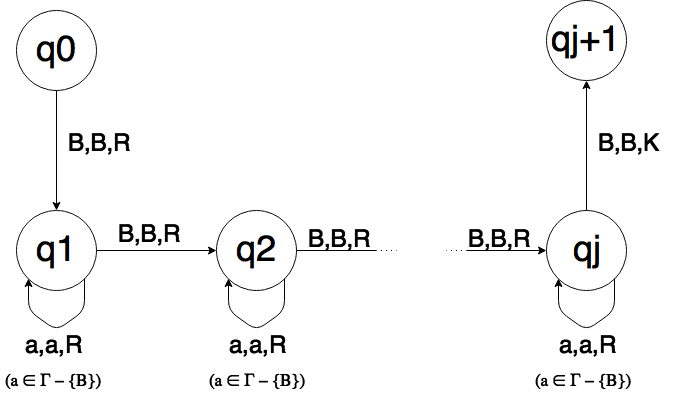
\includegraphics[scale=0.4]{graphics/figure_1.png}
        \end{figure}

        \PN Notar que:
    		\[
    		  \begin{array}{lcr}
            \alpha B \beta_{1} B \beta_{2} B \dotsc B \beta_{j} B \gamma &\overset{\ast}{\vdash}& \alpha B \beta_{1} B
              \beta_{2} B \dotsc B \beta_{j} B \gamma \\
            \ \ \uparrow && \uparrow \ \ \\
            \ \ q_{0} && q_{f} \ \
          \end{array}
    		\]

        \PN siempre que $\alpha, \gamma \in \Gamma ^{\ast}, \beta_{1}, \dotsc, \beta_{j} \in (\Gamma -\{B\})^{\ast}$.

      \item $I_{j}$ una máquina tal que:
    		\[
    		  \begin{array}{lcr}
            \alpha B \beta_{1} B
            \beta_{2} B \dotsc B \beta_{j} B \gamma &\overset{\ast}{\vdash}&  \alpha B \beta_{1} B \beta_{2} B \dotsc B
            \beta_{j} B \gamma \\
            \qquad\qquad\qquad\qquad \ \uparrow && \uparrow \qquad\qquad\qquad\qquad \ \\
            \qquad\qquad\qquad\qquad \ q_{0} && q_{f} \qquad\qquad\qquad\qquad \
          \end{array}
    		\]

        \PN siempre que $\alpha, \gamma \in \Gamma ^{\ast}, \beta_{1}, \dotsc, \beta_{j} \in (\Gamma -\{B\})^{\ast}$.

      \item $TD_{j}$ una máquina con un solo estado final $q_{f}$ y tal que:
    		\[
          \begin{array}{ccc}
            \alpha B \gamma &\overset{\ast}{\vdash} &\alpha B B \gamma \\
            \uparrow && \uparrow \ \ \\
            q_{0} & & q_{f} \ \
          \end{array}
        \]

        \PN cada vez que $\alpha, \gamma \in \Gamma^{\ast}$ y $\gamma$ tiene exactamente $j$ ocurrencias de $B$, es
        decir, la máquina $TD_{j}$ corre un espacio a la derecha todo el bloque $\gamma$ y agrega un blanco en el
        espacio que se genera a la izquierda de dicho bloque. Por ejemplo, para el caso de $\Sigma =\{\&\}$ podemos
        tomar $TD_{3}$ igual a la siguiente máquina:

        \begin{figure}[h]
          \centering
          \includegraphics[scale=0.4]{graphics/figure_3.png}
        \end{figure}

      \pagebreak
      \item $TI_{j}$ una máquina tal que:
    		\[
          \begin{array}{ccc}
            \alpha B \sigma \gamma &\overset{\ast}{\vdash}& \alpha B \gamma \\
            \uparrow \ && \uparrow \\
            q_{0} \ \ && q_{f}
          \end{array}
    	  \]

        \PN cada vez que $\alpha \in \Gamma ^{\ast }$, $\sigma \in \Gamma $ y $\gamma $ tiene exactamente $j$
        ocurrencias de $B$, es decir la máquina $TI_{j}$ corre un espacio a la izquierda todo el bloque $\gamma $ (por
        lo cual en el lugar de $\sigma $ queda el primer símbolo de $\gamma $).
    \end{itemize}

    \vspace{5mm}
    \PN Teniendo las máquinas auxiliares antes definidas podemos combinarlas para obtener las máquinas simuladoras de
    instrucciones. Por ejemplo $M_{i}^{a}$ puede ser la siguiente máquina:

    \begin{figure}[h]
      \centering
      \includegraphics[scale=0.4]{graphics/figure_4.png}
    \end{figure}

    \PN En la siguiente máquina, tenemos una posible forma de diseñar la máquina $IF_{i}^{a}$.

    \begin{figure}[h]
      \centering
      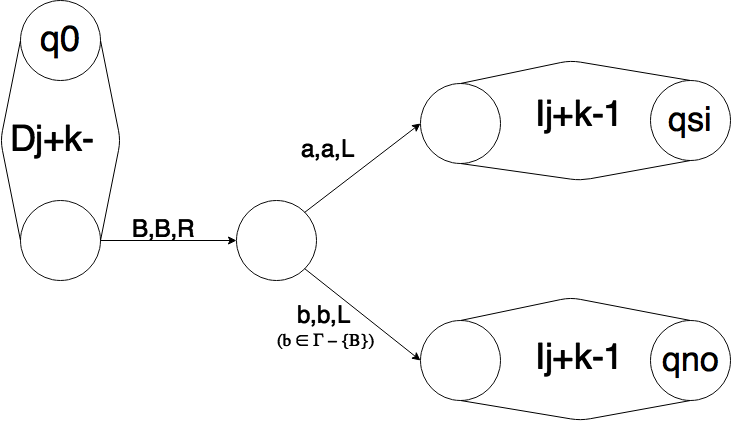
\includegraphics[scale=0.33]{graphics/figure_2.png}
    \end{figure}

    \pagebreak
    \PN En la siguiente máquina tenemos una posible forma de diseñar la máquina $M_{i\leftarrow j}^{\ast}$ para el caso
    $\Sigma = \{a,b\}$ y $i < j$:

    \begin{figure}[h]
      \centering
      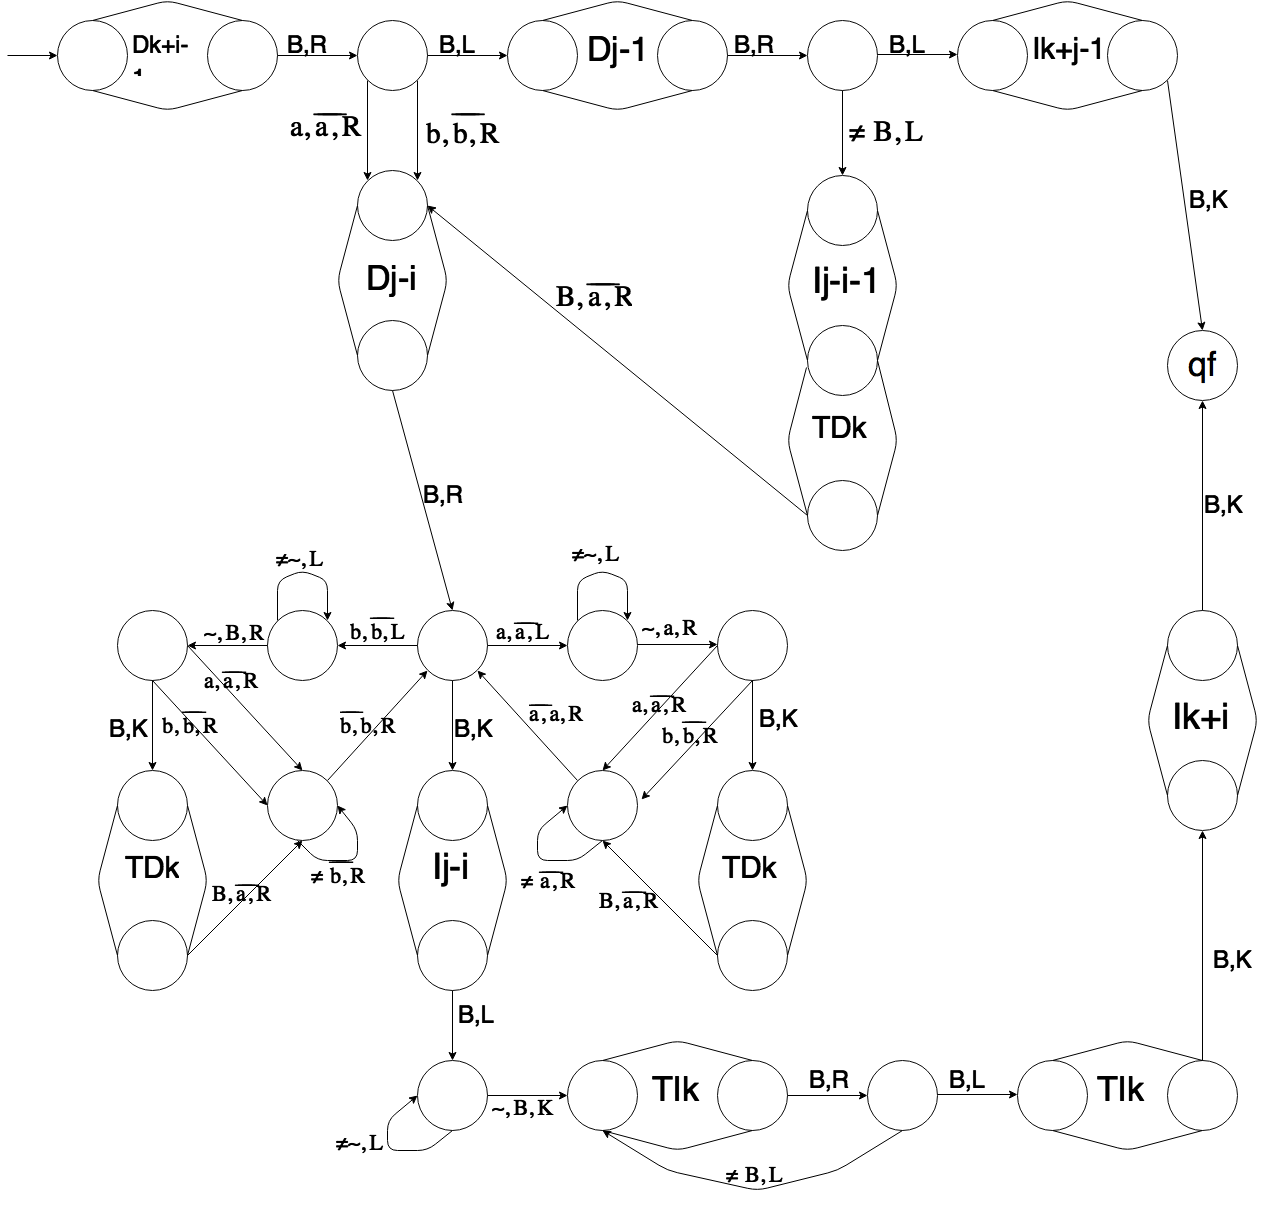
\includegraphics[scale=0.33]{graphics/figure_7.png}
    \end{figure}

    \pagebreak
    \PN Supongamos ahora que $\mathcal{P} = I_{1}, \dotsc, I_{n}$. Para cada $i = 1, \dotsc, n$, definiremos una máquina
    $M_{i}$ que simulará la instrucción $I_{i}$. Luego uniremos adecuadamente dichas máquinas para formar la máquina que
    simulará a $\mathcal{P}$.

		\begin{itemize}
			\item Si $Bas(I_{i})=\mathrm{N}\bar{j} \leftarrow \mathrm{N}\bar{j} + 1$ tomaremos $M_{i} = M_{j}^{+}$
	    \item Si $Bas(I_{i})=\mathrm{N}\bar{j} \leftarrow \mathrm{N}\bar{j} \dot{-} 1 $ tomaremos $M_{i} =
        M_{j}^{\dot{-}}$
	    \item Si $Bas(I_{i})=\mathrm{N}\bar{j} \leftarrow 0$ tomaremos $M_{i} = M_{j \leftarrow 0}$
	    \item Si $Bas(I_{i})=\mathrm{N}\bar{j} \leftarrow \mathrm{N}\bar{m}$ tomaremos $M_{i} = M_{j \leftarrow m}^{\#}$
	    \item Si $Bas(I_{i})=\mathrm{IF} \ \mathrm{N}\bar{j} \not = 0 \ \mathrm{GOTO} \ \mathrm{L}\bar{m}$ tomaremos
        $M_{i} = IF_{j}$
	    \item Si $Bas(I_{i})=\mathrm{P}\bar{j} \leftarrow \mathrm{P}\bar{j}.a$ tomaremos $M_{i}=M_{j}^{a}$
	    \item Si $Bas(I_{i})=\mathrm{P}\bar{j} \leftarrow \ ^{\curvearrowright} \mathrm{P}\bar{j}$ tomaremos $M_{i} =
        M_{j}^{\curvearrowright}$
	    \item Si $Bas(I_{i})=\mathrm{P}\bar{j} \leftarrow \varepsilon$ tomaremos $M_{i} = M_{j\leftarrow \varepsilon}$
	    \item Si $Bas(I_{i})=\mathrm{P}\bar{j} \leftarrow \mathrm{P}\bar{m}$ tomaremos $M_{i} = M_{j \leftarrow m}^{\ast}$
	    \item Si $Bas(I_{i})=\mathrm{IF} \ \mathrm{P}\bar{j} \ \mathrm{BEGINS} \ a \ \mathrm{GOTO} \ \mathrm{L}\bar{m}$
        tomaremos $M_{i} = IF_{j}^{a}$
	    \item Si $Bas(I_{i})=\mathrm{SKIP}$ tomaremos $M_{i} = M_{\mathrm{SKIP}}$.
	    \item Si $Bas(I_{i})=\mathrm{GOTO} \ \mathrm{L}\bar{m}$ tomaremos $M_{i} = M_{\mathrm{GOTO}}$
		\end{itemize}

    \PN Dado que la máquina $M_{i}$ puede tener uno o dos estados finales, se representará como se muestra en la
    siguiente figura:

    \begin{figure}[h]
      \centering
      \includegraphics[scale=0.4]{graphics/figure_5.png}
    \end{figure}

    \PN entendiendo que en el caso en que $M_{i}$ tiene un solo estado final, este esta representado por el circulo de
    abajo a la izquierda y en el caso en que $M_{i}$ tiene dos estados finales, el estado final corresponde al estado
    $q_{si}$ y el otro al estado $q_{no}$.

    \PN Para armar la máquina que simulará a $\mathcal{P}$, primero unimos las máquinas $M_{1}, \dotsc, M_{n}$ como lo
    muestra la siguiente figura:

    \begin{figure}[h]
      \centering
      \includegraphics[scale=0.5]{graphics/figure_6.png}
    \end{figure}

    \pagebreak
    \PN Luego para cada $i$ tal que $Bas(I_{i})$ es de la forma $\alpha \ \mathrm{GOTO} \ \mathrm{L}\bar{m}$, ligamos
    con una flecha de la forma:
		\[
      \underrightarrow{\qquad B,B,K \qquad}
		\]

    \vspace{5mm}
    \PN el estado final $q_{si}$ de la $M_{i}$ con el estado inicial de la $M_{h}$, donde $h$ es tal que $I_{h}$ es la
    primer instrucción que tiene label $\mathrm{L}\bar{m}$. Es intuitivamente claro que la máquina así obtenida cumple
    con lo requerido aunque una prueba formal de esto puede resultar extremadamente tediosa.
	\end{proof}

  \pagebreak
	% Theorem 85: Con prueba.
	\begin{theorem}
		\PN Si $f: D_{f} \subseteq \omega^{n} \times \Sigma^{\ast m} \rightarrow O$ es $\Sigma$-recursiva, entonces $f$ es
    $\Sigma$-Turing computable.
  \end{theorem}
  \begin{proof}
    \PN Dado que $f$ es $\Sigma$-computable, existe $\mathcal{P} \in \mathrm{Pro}^{\Sigma}$ el cual computa $f$. Se
    probará solamente el caso $O = \SIGMA$. Notar que cuando $\mathcal{P}$ termina, en el estado alcanzado, las
    variables numéricas tienen todas el valor $0$ y las alfabéticas distintas de $\mathrm{P}1$ todas el valor
    $\varepsilon$.

    \PN Sean:
    \begin{itemize}
      \item $M$ la máquina de Turing con unit dada por el \textbf{Lemma 84}, donde elegimos el número $k$ con la
        propiedad adicional de ser mayor que $n$ y $m$.

      \item $M_{1}$ una máquina tal que para cada $(\vec{x},\vec{\alpha}) \in \omega^{n} \times \Sigma^{\ast m}$
      	\[
          \left\lfloor q_{0} B \shortmid^{x_{1}} B \dotsc B \shortmid^{x_{n}} B \alpha_{1} B \dotsc B \alpha_{m} B
          \right\rfloor \overset{\ast}{\vdash}\left\lfloor q B \shortmid^{x_{1}} B \dotsc B \shortmid^{x_{n}}
          B^{k-n} B \alpha_{1} B \dotsc B \alpha_{m} B \right\rfloor
      	\]

        \PN donde $q_{0}$ es el estado inicial de $M_{1}$ y $q$ es un estado tal que $\delta(q,\sigma) =
        \emptyset$, para cada $\sigma$.

      \item $M_{2}$ una máquina tal que para cada $\alpha \in \SIGMA$
      	\[
          \left\lfloor q_{0} B^{k+1} \alpha \right\rfloor \overset{\ast}{\vdash} \left\lfloor q B \alpha
          \right\rfloor
      	\]

        \PN donde $q_{0}$ es el estado inicial de $M_{2}$ y $q$ es un estado tal que $\delta(q,\sigma) =
        \emptyset$, para cada $\sigma$.
    \end{itemize}

    \PN Notar que la concatenación de $M_{1}$, $M$ y $M_{2}$, en ese orden, produce una máquina de Turing la cual
    computa $f$.
	\end{proof}

  % Theorem 86: Nada.
  \begin{theorem}
    \PN Este teorema no se evalua.
  \end{theorem}
